\paragraph{}
Z gradientnim spustom i"s"cemo minimum ali pa maksimum neke funkcije, to pomeni kje ima funkcija najve"cjo oziroma najmanj"so vrednost. Gradientni spust je zelo primitivna metoda, pri kateri se preprosto premikamo v smer kamor funkcija nara"s"ca oziroma pada.

\paragraph{}
To si lahko predstavljamo s pomo"cjo slepega "cloveka, ki "zeli priti na vrh Golovca. Ko bo na"s "clovek, poimenujmo ga Lojze, na neki to"cki hriba, ne bo videl v katero smer mora hoditi (ker je slep), "cutil pa bo kako strm je hrib in v katero smer hrib nara"sca, v katero pa pada. Ker ho"ce priti na vrh, bo korak vsakokrat naredil v smer, v kateri je podlaga najbolj strma. Na za"cetku, ko je hrib bolj strm, bo Lojze naredil ve"cji korak, ko pa se bo pribli"zeval vrhu in bo hrib postajal manj strm, pa bo delal manj"se korake, ker se lahko druga"ce zgodi, da bo prestopil vrh in se zna"sel na drugi strani Golovca.

\paragraph{}
Z gradientnim spustom se torej premikamo v smer, v katero funkcija pada. Gradient te funkcije predstavlja smer, v katero funkcija pada oziroma nara"s"ca. Preden nadaljujemo z gradientom, si moramo ogledati kdaj funkcija pada in kdaj nara"s"ca.

\subsection*{Odvod}
\paragraph{}
Kot smo "ze omenili, nam gradient predstavlja strmino funkcije. Preden se lahko naprej pogovarjamo o gradientnem spust, potrebujemo definirati strmino funkcije.

\paragraph{}
Odvod neke funkcije $f(x)$ je strmina te funkcije v to"cki $x$. Odvod je pozitiven "ce funkcija nara"sca in negativen "ce funkcija pada. Ve"cji kot je odvod, bolj strma je funkcija v dani to"cki. Odvod funkcije $f(x)$, ki ga ozna"cimo z $f'(x)$, nam torej pove, kakšen je koeficient tangente na graf fukncije $ f(x) $ v točki $x$.


\begin{figure}[!h]
	\centering
	\caption{Odvod}
	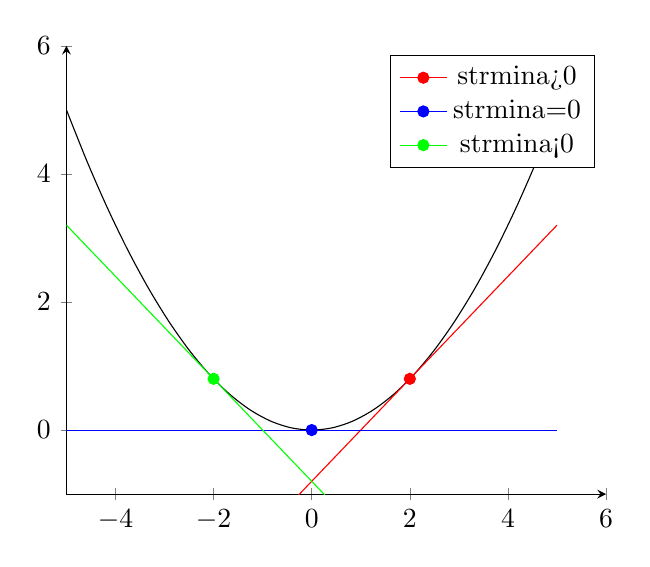
\begin{tikzpicture}
	\begin{axis}[axis lines=left, xmin=-5, xmax=6, ymin=-1, ymax=6]
	\addplot[color=black, smooth]{0.2*x^2};

	\addplot[color=red]{0.8*x - 0.8};
	\addplot[color=red, mark=*] coordinates {(2, 0.8)};

	\addplot[color=blue]{0};
	\addplot[color=blue, mark=*] coordinates {(0, 0)};

	\addplot[color=green]{-0.8*x - 0.8};
	\addplot[color=green, mark=*] coordinates {(-2, 0.8)};
	\legend{,,strmina>0,,strmina=0,,strmina<0}
	\end{axis}
	\end{tikzpicture}
\end{figure}


\subsection*{Malo o funkcijah}
\paragraph{}
Celo "zivljenje smo zapisavoli funkcije kot $f(x)$. Ta zapis nam predstavlja funkcijo, ki je odvisna od parametra $x$. To pomeni, da nam za vsak dani $x$ priredi novo "stevilko. "Ce "zelimo narisati graf take funkcije, uporabimo 2D koordinatni sistem in nanj nari"semo to"cke, ki nam jih da funkcija, to pomeni urejene pare $(x, f(x))$.

\paragraph{}
Ker pa smo v svobodni dr"zavi, nam ni prepovedano, da bi bila funkcija odvisna od ve"c parametrov. Funkcijo odvisno od dveh parametrov bi zapisali kot $f(x,y)$. Taki funkciji podamo 2 "stevilki, $x$ in $y$, vrne pa nam eno "stevilko. "Ce "zelimo narisati graf take funkcije potrebujemo 3D koordinatni sistem. Za vsako to"cko $T(x,y)$, bi nam taka funkcija priredila novo "stevilko, ki bi v tem koordinatnem sistemu predstavljala vi"sino, to je vrednost na $z$ osi. Primer take funkcije je:
\[f(x,y) = \frac{\sin \sqrt{x^2 + y^2}}{\sqrt{x^2 + y^2}} \]

$\sqrt{x^2 + y^2}$ predstavlja oddaljenost to"cke, ki jo podamo funkciji od izhodi"s"ca.

\begin{figure}[h!]
	\centering
	\caption{3D funkcija}
	\begin{tikzpicture}
	\begin{axis}[
	hide axis,
	colormap/cool,
	]
	%\addplot3[
	%	mesh,
	%	samples=50,
	%	domain=-8:8,
	%]
	%{sin(deg(sqrt(x^2+y^2)))/sqrt(x^2+y^2)};
	\legend{$\frac{\sin r}{r}$}
	\end{axis}
	\end{tikzpicture}
\end{figure}

Funkcija je seveda lahko odvisna tudi od ve"c spremenljivk. Takih funkcij pa ne moremo narisati, ker bi "ze za funkcijo odvisno od treh spremenljivk, potrebovali 4 dimenzionalni prostor.

\paragraph{}
Glede na to da smo "se vedno v svobodni dr"zavi, se lahko pri parametrih funkcije poigramo tudi z njihovim poimenovanjem. Nikjer ne pi"se, da ne smemo na mesto $x$ uporabljati $a$ in da na"sa funkcija ne sme izgledati kot $f(a)$. To seveda velja tudi za funkcije, ki vzamejo ve"parametrov, tako da lahko namest $f(x,y)$ pi"semo $f(a,b)$. Funkcijo katere graf je narisan od zgoraj, bi lahko potemtakem zapisali kot:
\[f(a,b) = \frac{\sin \sqrt{a^2 + b^2}}{\sqrt{a^2 + b^2}} \]

\paragraph{}
Definirali smo "ze napako premice za dane to"cke. Ker sedaj vemo, da je funkcija odvisna od ve"cih spremenljivk in da ni nujno da sta ti spremenljivki $x$ in $y$, lahko ugotovimo, da je na"sa napaka funkcija, ki je odvisna od spremenljivk $a$ in $b$. Druga"ce seveda ne more biti, ker imamo "ze podano skupino to"ck, to pomeni $x$ in $y$, za katere "zelimo najti premico, ki se jim prilega, tako da vse kar lahko spreminjamo v na"si funkciji napake sta parametra $a$ in $b$.

\subsection*{Delni odvod}
\paragraph{}
Pri funkciji, ki je odvisna od ve"cih parametrov se zakomplicira tudi odvod. Tako funkcijo moramo odvajati po vsaki spremenljivki posebej, kar pomeni da potrebujemo funkcijo $f(x,y)$ odvajati po $x$ in po $y$. S tem dobimo dva odvoda. Odvod po $x$ nam pove kako funkcija nara"s"ca oziroma po $x$ osi, odvod po $y$ pa nam seveda pove kako funkcija nara"s"ca oziroma pada po $y$ osi. Takemu odvodu re"cemo delni odvod, zapi"semo pa ga kot $\frac{\partial f(x,y)}{\partial x}$ za delni odvod po $x$ in $\frac{\partial f(x,y)}{\partial y}$ za delni odvod po $y$.

\paragraph{}
Za trenutek se vrnimo na za"cetni problem, ki nas je pripeljal do sem. "Zelelimo najti tako premico, ki se najbolj prilega vsem danim to"ckam. Definirali smo "ze skupno napako in ugotovili da je na"sa napaka funkcija, ki je odvisna od spremenjivk $a$ in $b$. Sedaj lahko pora"cunamo, kako strma je na"sa napaka za dani $a$ in $b$ po parametru $a$ in kako strma je po parametru $b$. Druga"ce povedano, izra"cunamo lahko delni odvod napake po $a$ in delni odvod napake po $b$.
$$\frac{\partial \varepsilon}{\partial a} =
\sum_{i=1}^{N} 2 \frac{\partial (a x_i + b - y_i)}{\partial a} =
2 \sum_{i=1}^{N} (a x_i + b - y_i)x_i$$

$$\frac{\partial \varepsilon}{\partial b} =
\sum_{i=1}^{N} 2 \frac{\partial (a x_i + b - y_i)}{\partial b} =
2 \sum_{i=1}^{N} (a x_i + b - y_i)\cdot1 = 2 \sum_{i=1}^{N} (a x_i + b - y_i)$$

\subsection*{Gradient}
\paragraph{}
Gradient neke funkcije je vektor, ki ka"ze v smer nara"s"canja te funkcije. Gradient funkcije $f$ ozna"cimo z $\nabla f$. Pri funkciji z enim parametrom ($f(x)$), ima gradient te funkcije samo eno komponento, to je odvod funkcije $f(x)$. To zapi"semo kot:
\[\nabla f = \begin{pmatrix}f'\end{pmatrix} \]

\paragraph{}
"Ce je funkcija odvisna od dveh spremenljivk, je vsaka komponenta gradienta en delni odvod. To pomeni, da nam prva komponenta gradienta pove kam nara"s"ca funkcija in kako strma je glede na prvi parameter, druga komponenta gradienta pa nam pove kam nara"s"ca funkcija in kako strma je glede na drugi parameter funkcije.

\paragraph{}
Za la"zjo predstavo si oglejmo gradient funkcije $f(x,y)$. Prva komponenta tega gradienta nam bo povedala strmino funkcije v smeri $x$ osi, druga komponenta tega gradienta pa nam pove strmino funkcije v smeri $y$ osi.

\paragraph{}
V splo"snem lahko gradient funkcije $f$, ki je odvisna od $n$ parametrov zapi"semo kot:
\[\nabla f = \begin{pmatrix}
\frac{\partial f}{\partial x_1} &
\frac{\partial f}{\partial x_2} &
\frac{\partial f}{\partial x_2} &
\dots &
\frac{\partial f}{\partial x_n}
\end{pmatrix} \]

Gradient na"se napake bi izgledal takole:
\[\nabla \varepsilon = \begin{pmatrix}
\frac{\partial \varepsilon}{\partial a} &
\frac{\partial \varepsilon}{\partial b}
\end{pmatrix} \]

